\chapter{Review of mesh movement methods}

 In our knowledge, there are, broadly speaking, two types of methods to achieve movement of the interior nodes knowing the movement of the boundary nodes. The first type uses models based on mechanics to try to achieve valid mesh movement. Examples of this type are lineal spring analogy \cite{mm:batina}, torsion spring analogy \cite{mm:torsionsprings}, linear-elasticity (and variants thereof)\cite{curve:hartmann} and non-linear elasticity \cite{curve:persson}. Each of these requires solution of a system of equations of size proportional to the number of mesh points to be moved. The linear-elasticity based models require solution of Poisson-type partial differential equations.
 
 The second type of technique to move the interior nodes involves \emph{interpolation} of the boundary displacement to interior nodes. Several methods exist; some examples are radial basis function (RBF) interpolation \cite{mm:rbf}, `explicit' interpolation \cite{mm:explicit}, and `Delaunay graph mapping' \cite{mm:dgm}. These methods do not involve any physics-based modeling of the mesh.
 
 \section{Elasticity-based methods}
 Elasticity-based methods are among the oldest mesh-movement methods in use. These include lineal spring analogy, torsional spring analogy, and various kinds of elastic solid mechanics analogies. These methods model the mesh as some kind of solid entity, impose a boundary displacement and solve equilibrium equations to propagate the motion to the interior nodes.
 
 \subsection{Spring analogies}
 
 Lineal spring analogy is the simplest method that can be used to move internal mesh points in response to movement of the boundary, invented by J.T. Batina. Each edge of the mesh is assumed to represent a lineal spring connecting the two nodes which make up the edge. The idea is that after imposing boundary movement, the mesh is allowed to ``go to equilibrium". At every mesh point, we have
 \begin{equation}
 \sum_j k_{ij}(\Delta \mathbf{r}_i - \Delta \mathbf{r}_j) = \mathbf{0} \quad \forall i
 \label{spring}
 \end{equation}
 where $i$ ranges over all nodes, $j$ ranges over points surrounding node $i$ and $\Delta \mathbf{r}_i$ is the displacement of node $i$.
 $k_{ij}$ is the stiffness of the spring between nodes $i$ and $j$, which can be taken as
 \begin{equation}
 k_{ij} = \frac{1}{||\mathbf{r}_i - \mathbf{r}_j||}.
 \end{equation}
 
 This method is not reliable as it generates invalid elements (having zero or negative value of the Jacobian determinant of the reference-to-physical element mapping) for even relatively small displacements, depending on the mesh. However, for the application it was developed, it sometimes gives acceptable results. It is used, for example, by Mavriplis \emph{et. al.} \cite{appl:mavriplis} in an optimization problem involving inviscid flow only. It is also less computationally expensive compared to other elasticity-based methods.
 
 Note that separate problems are solved in each coordinate direction, which are uncoupled. It is the author's opinion that this is the main reason for its unreliability for many kinds of mesh and movement combinations. However, because of this, extension to 3D is trivial.
 
 The torsional spring analogy is an extension to the previous method, which adds torsional springs at each node in each element (see Farhat \emph{et.al.} \cite{mm:torsionsprings}).
 These torsional springs resist the relative angular motion between edges of an element. This leads to a substantially more robust movement. In the scheme of Farhat \emph{et. al.}, the problem is divided into two parts, one related to lineal spring analogy and one to the torsional spring analogy. The lineal spring model is not the same as that used by Batina; in this case the lineal spring model also leads to a coupled system which is more robust than the uncoupled scheme. The torsional part adds even more resistance to invalid elements. As shown in figure \ref{f:torsion}, the torsional spring analogy adds torsion springs at each node of each element. The stiffness of a torsion spring associated with a node of a certain element is a function of the angle formed by the edges of that element meeting at the node.
 
 \begin{figure}
 	\centering
 	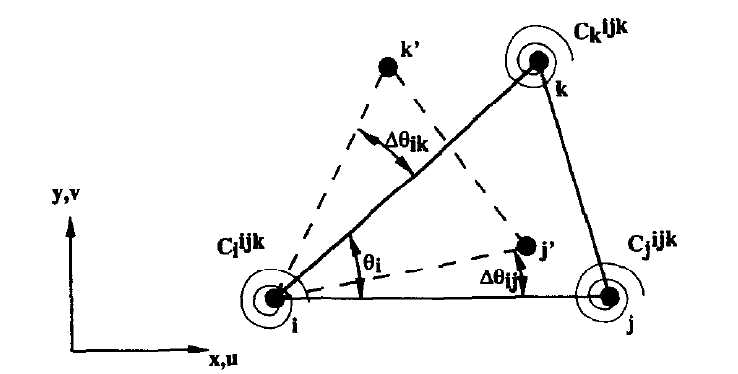
\includegraphics[scale=0.25]{torsionspring}
 	\caption{Movement of an element in torsion spring analogy; from \cite{mm:torsionsprings}}
 	\label{f:torsion}
 \end{figure}
 
 While this method is significantly more robust than the lineal spring analogy of Batina, it is also much more computationally expensive. A coupled system of $n_{dim} N_n$ equations must be solved, where $N_n$ is the number of nodes that are to be moved in the mesh and $n_{dim}$ is the physical spatial dimension of the problem.
 
 \subsection{Elastic solid analogy}
 
 The deformable elastic solid analogy, employing the equations of (linear or non-linear) elasticity, is one of the widely-used mesh movement techniques. This class of schemes often lead to very robust mesh movement. The mesh is assumed to model a deformable solid body, which is then deformed according to the equations of solid mechanics, that is, linear or non-linear elasticity.
 
 \subsubsection{Linear elasticity}
 
 The simplest approach is linear elasticity.
 \begin{equation}
 \nabla \cdot \mathbf{\sigma}  = \mathbf{0} \quad \text{in} \, \Omega
 \end{equation}
 Assuming an isotropic material, the constitutive relation can be taken as
 \begin{equation}
 \bld{\sigma} = 2\mu\bld{\epsilon} + \lambda (\mathrm{tr}\boldsymbol{\epsilon}) \bld{I}
 \label{linelast:constt}
 \end{equation}
 where $\bld{\sigma}$ is the stress and $\bld{\epsilon}$ is the strain.
 Finally, the linear strain-displacement relation is given by
 \begin{equation}
 \bld{\epsilon} = \frac12 (\nabla\bld{u}+\nabla\bld{u}^T)
 \label{linelast:strain}
 \end{equation}
 where $\bld{u}$ is the displacement field, with Dirichlet boundary conditions (prescribed boundary displacement $\bld{u}_b$)
 \begin{equation}
 \bld{u} = \bld{u}_b \quad \text{on} \, \partial\Omega
 \end{equation}
 The weak form of this set of equations, solved by Galerkin finite element method (FEM) leads to a linear system of size $n_d N_n$, where $n_d$ is the dimension of the problem and $N_n$ is the number of nodes to be moved.
 
 \subsubsection{`Sitffened' linear elasticity}
 \label{subsec:stiffelast}
 While the basic linear elasticity scheme is adequate for some applications, it is not adequate for stretched, boundary-layer meshes for viscous flow, among others. The scheme is often modified by `stiffening' the mesh appropriately, so as to attain some control over the propagation of deformation into the interior of the mesh, as done, for instance, by Hartmann and Leicht \cite{curve:hartmann}. In their work, the material is stiffened based on the determinant of the local Jacobian matrix of the reference-to-physical mapping, that is to say smaller elements are stiffer than larger ones. If $\hat{\kappa}$ is the reference element corresponding to the physical element $\kappa$, the local bilinear form on $\kappa$ giving rise to the local stiffness matrix 
 \begin{equation}
 (\dots)_\Omega = \sum_{\kappa \in T_h} \int_{\kappa} \dots d\mathbf{x} = \sum_{\kappa \in T_h} \int_{\hat{\kappa}} \dots J_\kappa d\mathbf{x}
 \end{equation}
 is modified according to
 \begin{equation}
\int_{\hat{\kappa}} \dots J_\kappa d\mathbf{x} \quad \text{becomes} \int_{\hat{\kappa}} \dots J_\kappa \left(\frac{J_0}{J_\kappa}\right)^\chi d\mathbf{x}
 \end{equation}
 where $J_\kappa$ is the Jacobian of the reference-to-physical mapping of the element $\kappa$, $J_0$ is a reference Jacobian for the mesh and $\chi$ is a constant to be chosen.
 
 We could also use other stiffening criteria. In our work we have tried stiffening based on the shape quality metric (section \ref{sec:lin-mesh-quality}), but we find that the shape metric generally leads to unacceptable results, and the size-shape metric is worse than Jacobian-based stiffening. Perhaps some other metric could be formulated that works better. Further, we could stiffen cells based on distance from boundaries. This would require a fast, and not necessarily very accurate, boundary-distance estimation.
 
 \subsubsection{Nonlinear elasticity}
 
 Nonlinear elasticity is claimed to be a highly robust method for mesh movement by Persson and Peraire \cite{curve:persson}. As long as the mesh is fine enough to resolve the displacements, they claim that element validity is guaranteed. In their work, for non-linear elasticity, the constitutive equation \eqref{linelast:constt} and strain-displacement relation \eqref{linelast:strain} are replaced by the `neo-Hookean' constitutive model
 \begin{equation}
 \bld{P} = \mu ((\boldsymbol{F}^T\bld{F})\bld{F}^{-T} - \bld{F}^{-T}) + \lambda(\ln \det\bld{F})\bld{F}^{-T}
 \end{equation}
 where the deformation gradient $\bld{F}$ is given by
 \[
 \bld{F} = \frac{\partial\bld{x}}{\partial\bld{X}}.
 \]
 Here, $\bld{x}$ is the physical position vector of a point with coordinate $\bld{X}$ in the reference configuration. The system is solved using Newton-GMRES iterations.
 
 In our opinion, this method probably cannot be used in any unsteady moving-geometry simulations, as the cost will be prohibitive. However, it leads to good results for curved mesh generation, as can be seen in Persson and Peraire's work.
 
 The advantage of elasticity-based methods is that they can be made highly robust. Their disadvantage is that generally, the more robust the scheme, the more expensive it is. The cost of the system of equations that needs to be solved usually scales with the total number of mesh nodes to be moved; this can get very expensive for 3D viscous meshes. Further, the implementation is usually not very easy; different cell types require different treatments (different basis functions, for instance, in case of elastic-solid approaches) and extension from 2D to 3D may not be trivial (as in case of torsional springs).
 
 \section{Interpolation  Methods}
 Also called algebraic methods, these methods do not involve any physics-based modeling of the mesh. They are purely mathematical manipulations of the mesh. Unlike elasticity-based methods, schemes of this type tend to be fast and independent of mesh topology.
 
 \subsection{Delaunay graph mapping (DGM)}
 \label{sec:dgm}
 Developed by Liu, Qin and Xia \cite{mm:dgm}, DGM is a fast method of mesh movement. It consists of the following steps (see figure \ref{fig:dgmprocess}).
 \begin{itemize}
 	\item A Delaunay triangulation is constructed from the boundary points of the mesh. This triangulation is referred to as the Delaunay graph.
 	\item Each internal mesh point is located in the Delaunay graph, and its barycentric coordinates are calculated with respect to the Delaunay element it lies in.
 	\item Using the prescribed boundary displacements, the Delaunay graph is moved.
 	\item Using the calculated barycentric coordinates, the interior mesh points are mapped back to the deformed Delaunay elements keeping the barycentric coordinates constant, thus moving the mesh.
 \end{itemize}
 Thus, no linear system needs to be solved. The bulk of the work is in computing the Delaunay triangulation and traversing it, which can be done efficiently. We use the Bowyer-Watson algorithm to compute the Delaunay tessellation of the boundary points in both 2D and 3D \cite{bowyer}. Details of the exact algorithm used are provided in appendix A.
 
 \begin{figure}
 	\centering
 	\subfloat{
 		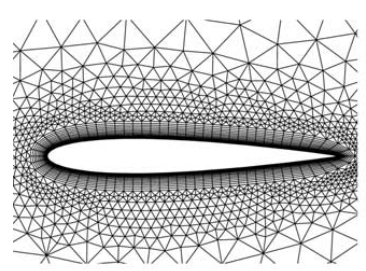
\includegraphics[scale=0.25]{dgm-mesh}
 	}
 	\subfloat{
 		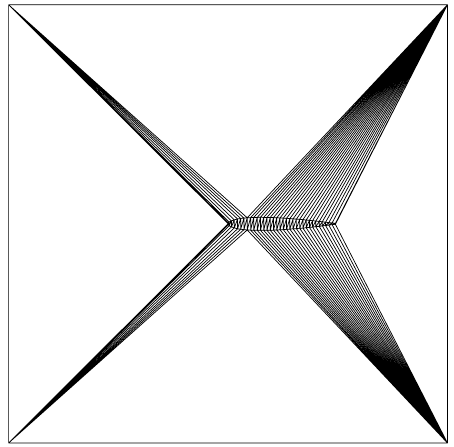
\includegraphics[scale=0.2]{dgm-dg}
 	}
 	\subfloat{
 		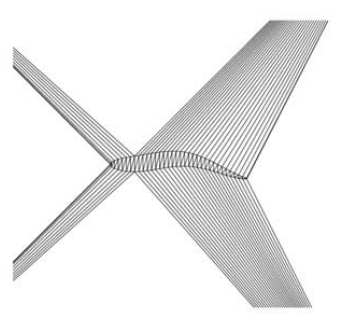
\includegraphics[scale=0.25]{dgm-moveddg}
 	}
 	\subfloat{
 		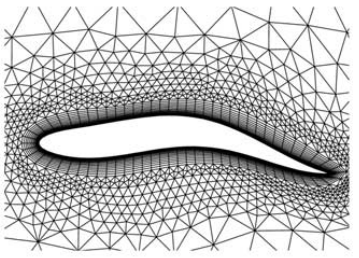
\includegraphics[scale=0.25]{dgm-movedmesh}
 	}
 	\caption{The DGM process (from left to right): original mesh, Delaunay graph, deformed Delaunay graph, deformed mesh (ref: \cite{mm:dgm})}
 	\label{fig:dgmprocess}
 \end{figure}
 
 This method results in a valid mesh as long as the boundary displacement does not invalidate the Delaunay graph itself. If the Delaunay graph becomes invalid, the displacement must be carried out in several steps. The Delaunay graph is re-computed each step, and thus much more boundary movement is possible without invalidating the sequence of Delaunay graphs.
 
 In our experiments, Delaunay graph mapping is not very robust when it comes to rotational motion, or otherwise very large deformation (see the results section).
 
 \subsection{Radial basis functions}
 
 Radial basis functions (RBFs) are radially-symmetric functions. They are used as a basis for the displacement field in the moving mesh \cite{mm:rbf}. Considering $n_b$ boundary points in the mesh, we express the displacement as
 
 \begin{equation}
 \mathbf{s}(\mathbf{x}) = \sum_{j=1}^{n_b} \mathbf{a}_j \phi(\lVert\mathbf{x} - \mathbf{x}_{bj}\rVert)
 \label{eqn:rbf}
 \end{equation}
 where $\mathbf{s}$ represents the displacement field, $\mathbf{x}$ is the position vector of any point in the domain, $\mathbf{x}_{bj}$ is the position of the $i$th boundary point, $\phi$ is a radial basis function, $\phi(\lVert\mathbf{x} - \mathbf{x}_{bj}\rVert)$ is the $j$th basis function for the displacement field, and $\mathbf{a}_j$ is the $j$th coordinate or coefficient in that basis.
 
 Since we know the displacements of the boundary nodes, we can solve for the coefficients $\mathbf{a}_j$ using
 \begin{equation}
 \mathbf{s}(\mathbf{x}_{ib}) = \sum_{j=1}^{n_b} \mathbf{a}_j \phi(\lVert\mathbf{x}_{bi} - \mathbf{x}_{bj}\rVert).
 \end{equation}
 
 In each coordinate direction, this leads to a system of $n_b$ equations in $n_b$ unknowns:
 \begin{equation}
 \mathbf{A}\mathbf{a}_k = \mathbf{s}_k
 \label{eqn:rbf_system}
 \end{equation}
 where the $(i,j)$ component of $\mathbf{A}$ is $\phi(\lVert\mathbf{x}_{bi} - \mathbf{x}_{bj} \rVert)$, $ \bld{a}_k \in \mathbb{R}^{n_b}$ is the coefficient vector in the $k$th direction and $\bld{s}_k \in \mathbb{R}^{n_b}$ is the vector of boundary displacements in the $k$th coordinate direction.
 
 In our implementation, we assemble $\mathbf{A}$ as a sparse matrix by evaluating the radial basis function between every pair of boundary points. This process can generally be parallelized easily. Once this linear system is solved, we need to evaluate equation \eqref{eqn:rbf} for each interior point, which requires one evaluation of the RBF for each interior point (in each direction). This too, can be parallelized easily.
 
 The quality of the final mesh depends on which RBF is used. Many kinds of RBFs have been used in literature \cite{mm:rbf, mm:rbf2}. In this work, we use Wendland's C2 function
 \begin{equation}
 \phi(x) = (1-x)^4(4x + 1),
 \end{equation}
 or rather, a modification,
 \begin{equation}
 \phi(x) = 
 \begin{cases}
 \left(1-\frac{x}{r_s}\right)^4\left(4\frac{x}{r_s} + 1\right) & x < r_s \\
 0 & x \geq r_s
 \end{cases}
 \end{equation}
 where $r_s$ is a real number called the `support radius'. This modified function has a compact support. In light of this, we see the matrix $\mathbf{A}$ is sparse if the support radius is less than the characteristic dimension of the domain. For curved mesh generation, this support radius can be kept quite small relative to the whole domain, giving us a very sparse linear system which is solved quite fast. Wendland's C2 function is claimed to be positive definite \cite{rbf:errorwendland} for 2D and 3D problems. This means that the RBF interpolation matrix must be positive definite, and must therefore be solvable quickly by conjugate gradient or Cholesky decomposition methods.
 
 The scaling of the argument by the support radius serves to make the value of the RBF 1.0 at the boundary. This means that points very close to the boundary will deform just like the boundary itself. This results in an essentially rigid motion of points very close to the boundary, which causes the near-boundary elements to retain their quality after the mesh movement. The support radius is chosen big enough to accommodate the expected deformation of the boundary, but small enough that the linear system is sparse. An algorithm to determine a good support radius will be very useful in this regard.
 
 The RBF method can be carried out in multiple steps; this is found to increase the quality of generated meshes in cases involving large rotational deformations (figure \ref{fig:wing-inviscid-rbf}), but not so much in others, such as curved mesh generation.
 
 \subsection[DG-RBF]{Interpolation using radial basis function on the Delaunay graph (DGRBF)}
 This method proposed by Wang, Qin and Zhao \cite{mm:dgrbf} combines both the Delaunay graph mapping and interpolation by RBF. The general scheme of the mesh movement is the same as in case of DGM, but with the important difference that interpolation is not done using barycentric coordinates of the nodes with respect to the Delaunay graph elements. Here, the interpolation is done via radial basis functions in each Delaunay graph element. The displacement of a node with initial position $\bld{x}$ is given by
 \begin{equation}
 \mathbf{s}(\mathbf{x}) = \sum_{j=1}^{n_t} \mathbf{a}_j \phi(\lVert\mathbf{x} - \mathbf{x}_{tj}\rVert)
 \label{eqn:dgrbf}
 \end{equation}
 where $\bld{x}_{tj}$ are positions of nodes of the Delaunay simplex that contains the node at $\bld{x}$, and $n_t$ is the number of nodes in that simplex (3 in 2D and 4 in 3D). We need to solve for the $\bld{a}_j$, the RBF coefficients, by solving a $3 \times 3$ system in 2D or a $4 \times 4$ system in 3D, in each Delaunay element.
 \begin{equation}
 \mathbf{s}(\mathbf{x}_{ti}) = \sum_{j=1}^{n_t} \mathbf{a}_j \phi(\lVert\mathbf{x}_{ti} - \mathbf{x}_{tj}\rVert).
 \label{eqn:dgrbfsys}
 \end{equation}
 
 DGRBF method provides flexibility in choosing the RBF and the support radius, and with a good choice of these, robust mesh movement can be achieved for translational motion and possibly some other kinds of deformation. It has been observed in \cite{mm:dgrbf} and in our tests, that interpolation of displacements by DGRBF often does not give very good results for large rotational deformations. The remedy for this is to interpolate the rotational angles instead of the displacements directly, and then calculate the displacements at each interior node using these interpolated rotation angles using the rotation matrix. For example, in 2D,
 \begin{align}
 x_{new} &= (x-x_0)\cos a_z - (y-y_0)\sin a_z + x_0 \\
 y_{new} &= (x-x_0)\sin a_z + (y-y_0)\cos a_z + y_0
 \end{align}
 where $(x_0,y_0)$ is the center of rotation, and $a_z$ is the interpolated rotation angle at the node in question. For interpolation of the angles, the same formulae \eqref{eqn:dgrbf} and \eqref{eqn:dgrbfsys} are used, with the rotation angles replacing the displacements. Angle interpolation can be combined with displacement interpolation for problems involving both translation and rotation. This angle interpolation scheme, and its combination with the displacement interpolation scheme, is referred to as `DGRBF2' in \cite{mm:dgrbf}.
 
 \subsection{`Improved' Delaunay graph mapping}
 \label{sec:hybriddg}
 If the Delaunay graph (DG) lines are not approximately normal to the boundary, there can sometimes be issues with mesh movement. Mesh lines tend to be normal to the boundary for physical and numerical reasons. If Delaunay graph lines make very small or very large angles (compared to 90 degrees) with the boundary, successive interior nodes on the same mesh line can lie in different DG triangles. This would cause non-smooth displacement of interior mesh nodes; an example is presented in detail in section \ref{subsec:dgmunsuitable}.
 
 One way of improving this method, that was considered by the author and Dr Hong Luo, was to include a few interior mesh points in the Delaunay graph such that the Delaunay graph lines stayed approximately normal to the boundary near it. For example, a layer of nodes could be chosen around each component of a 3-component airfoil (figure \ref{fig:wmesh}) such that each airfoil boundary gets approximately normal Delaunay graph lines. This method would require movement of the interior Delaunay graph nodes by a different method, such as RBF or linear elasticity. Since the number of these interior nodes in the Delaunay graph is very small, solution of the RBF or linear elasticity problems could be done quickly.
 
 % ADD PICTURE HERE
 
 Xiao et. al. present a very similar method \cite{mm:hybriddg}. Instead of choosing interior Delaunay graph points from among the interior mesh points, they generate a `background' coarse mesh to serve as the Delaunay graph (DG). The motion of the DG is obtained using Batina's lineal spring analogy method \cite{mm:batina}.
 
 \section{Linear Mesh quality}
 \label{sec:lin-mesh-quality}
 In order to judge the effectiveness of mesh-movement methods, we need to measure the quality of the deformed mesh. Some mesh quality measures have been derived for linear 2D and 3D elements by Knupp \cite{qualknupp}. These include the relative size, shape and size-shape metrics for triangles and tetrahedra, and size, shape, skew, size-shape and size-skew metrics for quadrangles and hexahedra.
 
 The size metric distinguishes elements having very small or very large volume with respect to some reference volume. The shape metric identifies elements that have unequal edges or unequal angles between edges; it is independent of size of the element. Finally, the skew metric is a measure of unequal angles between edges of the element only, irrespective of lengths of edges and volume of element. The skew metric is different from shape in case of non-simplicial (like quadrangular and hexahedral) elements. While dealing with quadrilaterals, we use the skew metric. This is because for boundary layer meshes, cells with high aspect-ratios are desired, but they have poor shape metric. For triangular meshes, cells with high aspect-ratio must have very unequal interior angles too, leaving no difference between shape and skew.
 
 All metrics are normalized so that they are 1.0 for ideal elements with regard to the characteristic they measure, and they are 0.0 for degenerate elements. 
 
